
\chapter{Manual}
\label{cha:manual}

The project code and documentation is hosted on the \texttt{masci-tools}
repository \cite{masci-tools} under the branch
\href{https://github.com/JuDFTteam/masci-tools/tree/studentproject18ws}{\texttt{studentproject18ws}}.
All of the project code resides in the folders \texttt{binder} (for the Web
Frontend Demo) and \texttt{studentproject18w} (all code and documentation). The
\texttt{README.md} serves as the manual. Therefore, the remaining part of this
chapter is a \TeX{}-ified version of that \texttt{README.md}.

\vspace{3em}
\hdashrule{\textwidth}{2pt}{2pt}
%% BEGIN TEXIFIED MANUAL ========================================
%%
%% JW: manual changes necessary to the TeX-ified version:
%% - figure -> figure*
%% - texttt{long} -> path{long}
%% - replace code sections 'Tok' with lstlisting
%%

SiScLab 2018 Student Project \textbf{Analysis Tool for Materials
Design}. Written in Python3.

Authors: \href{https://github.com/Irratzo}{Johannes Wasmer},
\href{https://github.com/ChristianPartmann}{Christian Partmann}, and
\href{https://github.com/PraneethKatta}{Praneeth Katta}.

\section{Overview}\label{overview}

This subfolder \texttt{studentproject18ws} is currently a largely
independent side-project accompanying the main module
\texttt{masci-tools}. It was created in a student project, and consists
of three submodules:

\begin{itemize}
\tightlist
\item
  preprocessor: a HDF reader interface, and one implementation for Fleur
  band structure simulation output
\item
  visualization: a plotting interface, and one implementation for Fleur
  bandstructure+DOS plots
\item
  frontends: a Desktop GUI and a Web Dashboard (Tk and Jupyter) for
  interactive Fleur bandDOS plots.
\end{itemize}

A more thorough description and example use cases can be found in the
project \href{./doc/report.pdf}{report} and
\href{./doc/presentation.pdf}{presentation}.

\begin{figure*}
\centering
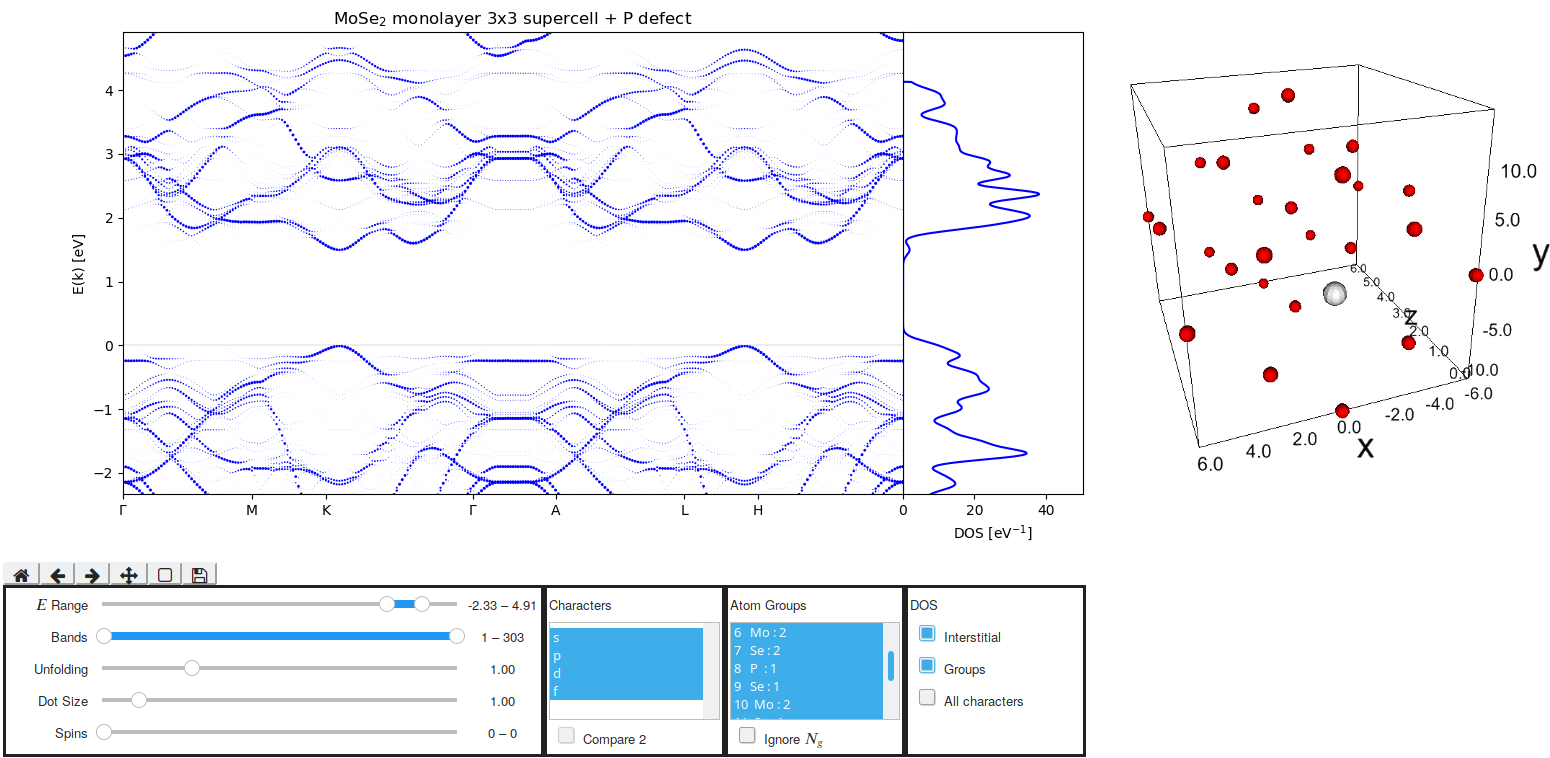
\includegraphics{./readme/web_frontend.png}
\caption{}
\end{figure*}

\section{For Frontend Users}\label{for-frontend-users}

The Desktop GUI executable can be received from the developers on
request. Otherwise, it can be built using
\href{https://www.pyinstaller.org/}{PyInstaller} from this repo.

The Web Frontend is a Jupyter Dashboard. It is in experimental phase (no
fileupload yet). You can try it out
\href{https://mybinder.org/v2/gh/JuDFTteam/masci-tools/studentproject18ws?filepath=studentproject18w\%2Ffrontend\%2Fjupyter\%2Fdemo\%2Fbinder_demo.ipynb}{here
on Binder}. You can run it locally (see developer section). If you have
an \href{https://aiidalab.materialscloud.org/hub/login}{AiiDaLab
account}: the dashboard is planned to be published as an app there.

\section{For Developers}\label{for-developers}

\subsection{Installation}\label{installation}

Though \texttt{masci-tools} is availabe via PyPI, there is currently no
plan to integrate \texttt{studentproject18ws}. If you want to use it in
your code, clone the repo, use it in an IDE, or append the path to your
\texttt{sys.path}:

\begin{lstlisting}[language=python, style=code]
import sys
if path_repo not in sys.path:
    sys.path.append(path_repo)
    
# now import works
from studentproject18w.hdf.reader import Reader
# ...
\end{lstlisting}

\subsubsection{Create project virtual
environment}\label{create-project-virtual-environment}

With conda (recommended): -
\href{https://www.anaconda.com/download}{Install Anaconda (3
recommended)} - Install the environment \texttt{masci-stupro} with the
necessary and recommended dependencies:


\begin{lstlisting}[language=bash, style=code]
conda create -f environment.yml
source activate masci-stupro
\end{lstlisting}

With virtualenv (untested):

\begin{lstlisting}[language=bash, style=code]
virtualenv masci-stupro
source masci-stupro/bin/activate
pip install -r requirements_pip.txt # install requirements
\end{lstlisting}

\subsection{Programmatic use}\label{programmatic-use}

In this example, a Fleur HDF file is preprocessed using the Recipe
\texttt{FleurBands}. The resulting output \texttt{data} with the extracted and
transformed HDF datasets and attached load methods (Extract-Transform-Load) is
then passed to a plotter, alongside some DOS CSV files for a bandstructure plot
using \texttt{matplotlib} as backend library.

\begin{lstlisting}[language=python, style=code]
import matplotlib.pyplot as plt
from studentproject18w.hdf.reader import Reader
from studentproject18w.hdf.recipes import Recipes
from studentproject18w.plot.matplot import BandDOSPlot

data = None
reader = Reader(filepath=filepath_hdf)
with reader as h5file:
    data = reader.read(recipe=Recipes.FleurBands)
    #
    # Note:
    # Inside the with statement (context manager),
    # all data attributes that are type h5py Dataset are available (in-file access)
    # When the statement is left,the HDF5 file gets closed and the datasets are closed.
    #
    # Use data outside the with-statement (in-memory access: all HDF5 datasets converted to numpy ndarrays):
    data.move_datasets_to_memory()

plotter = BandDOSPlot(plt, data, filepaths_dos)
(fig, ax_bands, ax_dos) = plter.setup_figure(fig_ratio=[12,6], fig_scale=1, fig_title="BandDOS")
data_selection = some_selection_process()
plotter.plot_bandDOS(*data_selection)
plt.show()
\end{lstlisting}


\subsection{Try out Web Frontend
locally}\label{try-out-web-frontend-locally}

The demo notebook with the Dashboard is
\url{studentproject18w/frontend/jupyter/demo/demo.ipynb}.

\subsubsection{If using Jupyter Notebook
Notebook}\label{if-using-jupyter-notebook}

If using Windows, omit keyword \texttt{source}.

\begin{lstlisting}[language=bash, style=code]
source activate masci-stupro
cd mypath/masci-tools/studentproject18ws/
jupyter-notebook .
# if Home is not set to this dir, try this instead:
# /home/you/anaconda3/envs/myenv/bin/python /home/you/anaconda3/envs/myenv/bin/jupyter-notebook .
\end{lstlisting}


\subsubsection{If using Jupyter Lab}\label{if-using-jupyter-lab}

Additional installation step needed:

\begin{lstlisting}[language=bash, style=code]
source activate masci-stupro
jupyter labextension install @jupyter-widgets/jupyterlab-manager jupyter-matplotlib ipyvolume
cd mypath/masci-tools/studentproject18ws/
jupyter-lab
\end{lstlisting}

\subsection{To-do list for publishing the Web
Frontend}\label{to-do-list-for-publishing-the-web-frontend}

\begin{itemize}
\tightlist
\item
  (recommended: create \texttt{frontend/jupyter/Dashboard.py} widget and
  put code of
  \href{./frontend/jupyter/demo/demo_backend.ipynb}{demo\_back.ipynb}
  notebook inside it. Use
  \href{https://github.com/aiidalab/aiidalab-widgets-base/blob/master/aiidalab_widgets_base/structures.py}{aiidalab-widgets-base
  \textgreater{} StructureUploadWidget} as a template. Create
  \texttt{frontend/jupyter/Dashboard.ipynb} notebook. Use
  \href{https://github.com/aiidalab/aiidalab-widgets-base/blob/master/structures.ipynb}{StructureUploadWidget
  Demo Notebook} as a template.)
\item
  Add \href{https://pypi.org/project/fileupload/}{fileupload} to widget
  (again, like in StructureUploadWidget. See
  \href{./frontend/jupyter/demo/binder_fileupload_test.ipynb}{binder\_fileupload\_test.ipynb}
  notebook for a demo that works with Binder.)
\item
  Now the Web Frontend should work on Binder.
\item
  For publishing the app on AiiDA Lab, the app has to be registered in
  the
  \href{https://github.com/aiidalab/aiidalab-registry}{aiidalab-registry}.

  \begin{itemize}
  \tightlist
  \item
    The project code is in Python3, but aiidalab requires Python2. So
    the code has to first be backported by hand using the
    \texttt{future} package. If this takes too long, maybe try the tool
    \href{https://pypi.org/project/3to2/}{3to2}.
  \item
    Use the simplest app in the registry,
    \href{https://github.com/aiidalab/aiidalab-units}{aiidalab-units} as
    a template. Adapt code.
  \item
    Try it out first in the
    \href{https://www.materialscloud.org/work/quantum-mobile}{Quantum
    Mobile Virtual Machine}, which has aiidalab installed and
    configured. Else try it in a virtual environment with
    \href{https://pypi.org/project/aiidalab/}{aiidalab} installed from
    PyPI.
  \item
    Register the app.
  \end{itemize}
\end{itemize}

Note: other publishing options besides Binder and AiiDALab are listed
\href{https://github.com/markusschanta/awesome-jupyter}{here}. For
instance, \href{http://colab.research.google.com/}{Google Colaboratory}
is a free Notebook hosting service that allows file upload.


%% FINISH TEXIFIED MANUAL ========================================
\hdashrule{\textwidth}{2pt}{2pt}






%% =========================================================
%%% Manuals Chapter OLD VERSION ============================
%% =========================================================
% \section{Frontends User Manual}
% \label{sec:user-manual}

% \subsection{System Requirements \& Installation}
% \label{sec:system-requirements}

% The Desktop Frontend is distributed as an executable file. 

% \subsection{Input Data Formats}
% \label{sec:input-data-formats}

% \subsection{GUI Usage}
% \label{sec:gui-usage}

% The Desktop and Web Frontend are functionally identical and use the same
% graphical descriptors. Thus these points hold true for both alike.

% Instead of dragging the sliders, values can be typed into their adjoining value
% displays as well.

% \textbf{TODO}: web frontend: binder or colab link

% \subsection{Troubleshooting}
% \label{sec:troubleshooting}


% \section{Developer Manual}
% \label{sec:developer-manual}

% At the time of this report, the package is written in Python 3. It is hosted on
% the \texttt{masci-tools} repository \cite{masci-tools} under the branch
% \href{https://github.com/JuDFTteam/masci-tools/tree/studentproject18ws}{\texttt{studentproject18ws}}.
% All of the project code resides in the folders \texttt{binder} (for the Web
% Frontend; see below) and \texttt{studentproject18w} (all code and
% documentation). The \texttt{README.md} contains the same installation
% instructions listed here.

% \subsection{Creating the project virtual environment}
% \label{sec:creat-proj-virt}

% \begin{lstlisting}[language=bash, style=code]
%     # if using conda (recommended)
%     conda create -f environment.yml
%     source activate 

%     # if using pip (untested)
    
% \end{lstlisting}

% \subsection{Creating Desktop Frontend Executables}
% \label{sec:creat-deskt-front}



% \subsection{Extending the Preprocessor}
% \label{sec:extend-prepr}

% \subsection{Extending the Visualization \& Frontends}
% \label{sec:extend-visu-}

% \textbf{TODO:} publish on aiidalab 

% \textbf{TODO:} hosting alternatives
% \begin{itemize}
% \item binder with example
% \item google colab (see jupy wiki or jupy awesome) \cite{jupyter-awesome}
% \item voila?
% \end{itemize}







%%% Local Variables:
%%% mode: latex
%%% TeX-master: "../report"
%%% End:
